\documentclass[11pt]{beamer}
\usetheme{Boadilla}
\usepackage[utf8]{inputenc}
\usepackage[spanish]{babel}
\usepackage{amsmath}
\usepackage{amsfonts}
\usepackage{amssymb}
\usepackage{graphicx}
\usepackage{subfig}

%%%%% Color institucional
\definecolor{MyBackground}{rgb}{1.0000,0.9451,0.6549}
\definecolor{itesm}{HTML}{0658a6}
\definecolor{lnppdos}{RGB}{59,124,188}
\definecolor{lnpptres}{RGB}{124,172,212}
%\definecolor{MyBackground}{RGB}{255,241,167}
%\setbeamercolor{background canvas}{bg=MyBackground}
\setbeamercolor*{palette primary}{bg=lnpptres, fg = black}
\setbeamercolor*{palette secondary}{bg=lnppdos, fg = white}
\setbeamercolor*{palette tertiary}{bg=itesm, fg = white}
\setbeamercolor{frametitle}{fg=itesm,bg=white}
\setbeamercolor{title}{fg=white,bg=itesm}
\setbeamercolor{caption name}{fg=itesm}
\setbeamercolor*{item}{fg=itesm}
\usepackage{xcolor}

%%%%%%
\title[Clase]{Programación probabilística y problemas inversos en ecuaciones diferenciales ordinarias}
\institute[EGTP]{Simulación de sistemas \\ Escuela de Gobierno y Transformación Pública, ITESM} 
\date{\today} 
\subject{Resultados} 
\titlegraphic{
\includegraphics[width=3cm]{images/egap}\hspace*{7.5cm}
}
%\title{Turing ODE}
%\setbeamercovered{transparent} 
%\setbeamertemplate{navigation symbols}{} 
%\logo{} 
%\institute{} 
%\date{} 
%\subject{} 
\begin{document}

\begin{frame}
\titlepage
\end{frame}

%\begin{frame}
%\tableofcontents
%\end{frame}

\begin{frame}
	\begin{figure}
		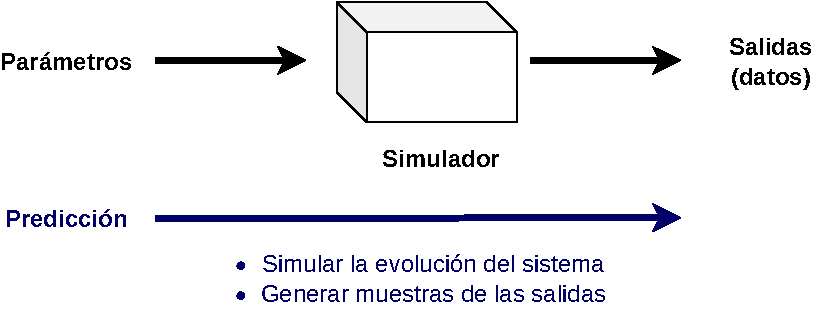
\includegraphics[scale=0.8]{images/turing_ode-simulators-1.pdf}
		\caption{\scriptsize Adaptado de Atılım Güneş Baydin, \textit{Probabilistic Programming for Inverse Problems in the Physical Sciences}. Recurso : \url{https://www.youtube.com/watch?v=E3_Ey0z068o}}
	\end{figure}
\end{frame}

\begin{frame}
	\begin{figure}
		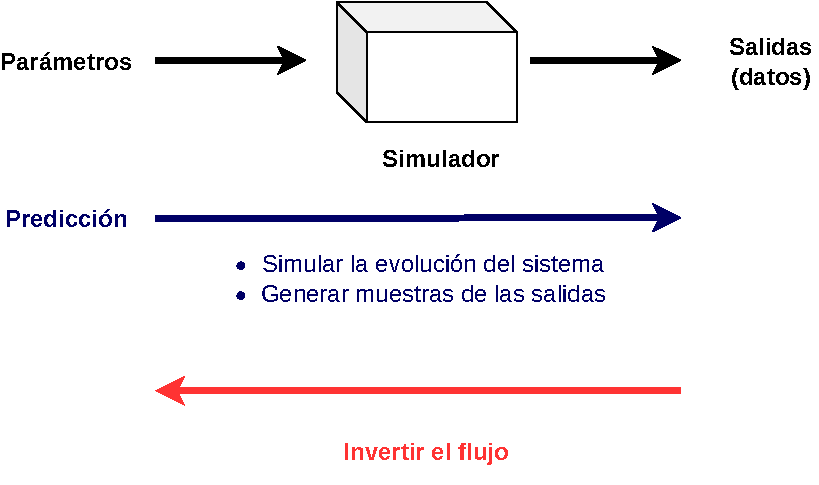
\includegraphics[scale=0.8]{images/turing_ode-simulators-2.pdf}
		\caption{\scriptsize Adaptado de Atılım Güneş Baydin, \textit{Probabilistic Programming for Inverse Problems in the Physical Sciences}. Recurso : \url{https://www.youtube.com/watch?v=E3_Ey0z068o}}
	\end{figure}
\end{frame}

\begin{frame}
	\begin{figure}
		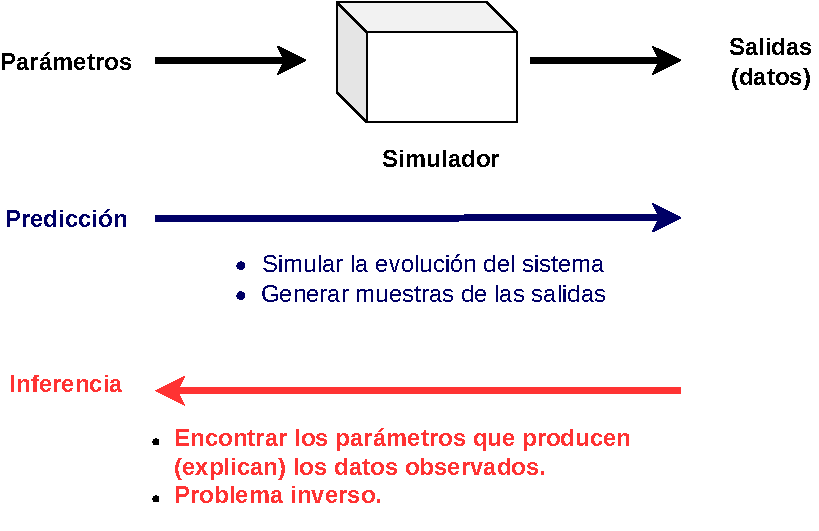
\includegraphics[scale=0.8]{images/turing_ode-simulators-3.pdf}
		\caption{\scriptsize Adaptado de Atılım Güneş Baydin, \textit{Probabilistic Programming for Inverse Problems in the Physical Sciences}. Recurso : \url{https://www.youtube.com/watch?v=E3_Ey0z068o}}
	\end{figure}
\end{frame}

\begin{frame}{Reconstrucción de redes}
	\begin{figure}
		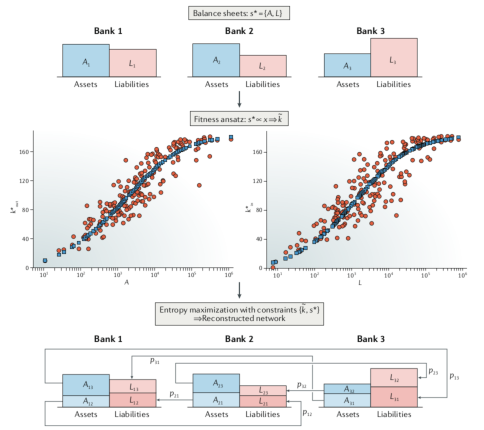
\includegraphics[scale=0.9]{images/financial_net}
		\caption{\tiny Tomado de Cimini, G., Squartini, T., Garlaschelli, D. \& Gabrielli, A Systemic risk analysis on reconstructed economic and
financial networks. Sci. Rep. 5, 15758 (2015).}
	\end{figure}
\end{frame}


\begin{frame}
	\begin{figure}
		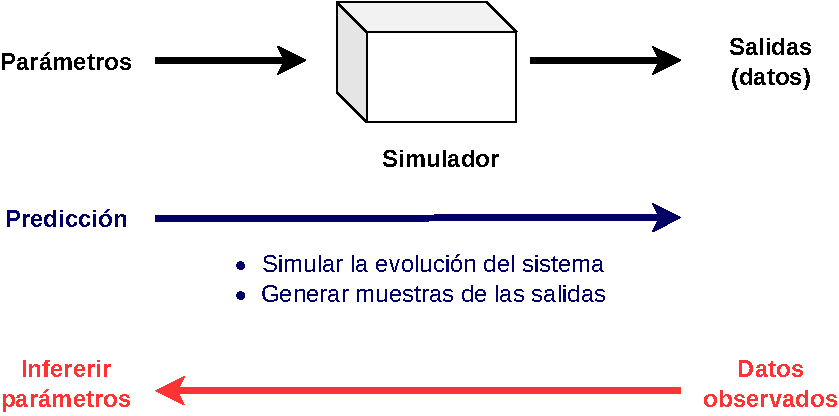
\includegraphics[scale=0.8]{images/turing_ode-simulators-4.pdf}
		\caption{\scriptsize Adaptado de Atılım Güneş Baydin, \textit{Probabilistic Programming for Inverse Problems in the Physical Sciences}. Recurso : \url{https://www.youtube.com/watch?v=E3_Ey0z068o}}
	\end{figure}
\end{frame}

\begin{frame}{Programación probabilística}
	\begin{columns}
\begin{column}{0.5\textwidth}

	\begin{itemize}
	\item Es un enfoque de aprendizaje de máquinas que permite escribir programas que representan modelos probabilísticos.
	\item La programación probabilística soporta declaraciones probabilísticas como declaración de variables aleatorias.
	\item Permite la inferencia (bayesiana) de parámetros condicionados en datos observados.
	\end{itemize}
\end{column}
\begin{column}{0.5\textwidth}
	\begin{figure}
		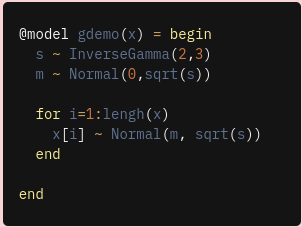
\includegraphics[scale=0.4]{images/prob_prog}
	\end{figure}
\end{column}

\end{columns}
\end{frame}

\begin{frame}{Frameworks para programación probabilística}
\begin{figure}%
 \subfloat[\centering Pyro]{{
\includegraphics[width=4cm]{images/pyro} }}%
 \qquad
 \subfloat[\centering Stan]{{
\includegraphics[width=4cm]{images/stan} }}%    \caption{2 Figures side by side}%
    \label{fig:example}%
\end{figure}
\end{frame}

\begin{frame}{Turing.jl }
	\begin{figure}
		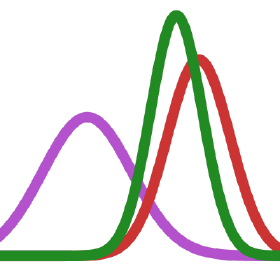
\includegraphics[scale=0.4]{images/turing}
		\caption{\url{https://turing.ml/stable/}}
	\end{figure}
\end{frame}

\begin{frame}{¿Por qué otro lenguaje de alto nivel?}


\begin{columns}
\begin{column}{0.5\textwidth}
	{\center \textbf{Características típicas}}
	
	\begin{itemize}
		\item Tipado dinámico. 
		\item Sintaxis de alto nivel.
		\item Open source.
		\item Built-in package manager.
	\end{itemize}
\end{column}
\begin{column}{0.5\textwidth}  %%<--- here
	{\center \textbf{Características novedosas}}
	\begin{itemize}
		\item Buen perfomance: tiempo de ejecución rápido.
		\item Compilación JIT (Just in Time) a nivel de función.
		\item En un porcentaje alto, Julia está escrito en Julia. 
		\item Metaprogramación (macros).
	\end{itemize}
\end{column}
\end{columns}

\end{frame}



\begin{frame}{Ecuaciones diferenciales ordinarias\footnote{Tomado de las notas de Ben Lampert sobre inferencia bayesiana \url{https://ben-lambert.com/bayesian-short-course/}}}

Realizamos experimentos donde se inoculan placas de agar con bacterias en el tiempo 0.
	\begin{figure}
		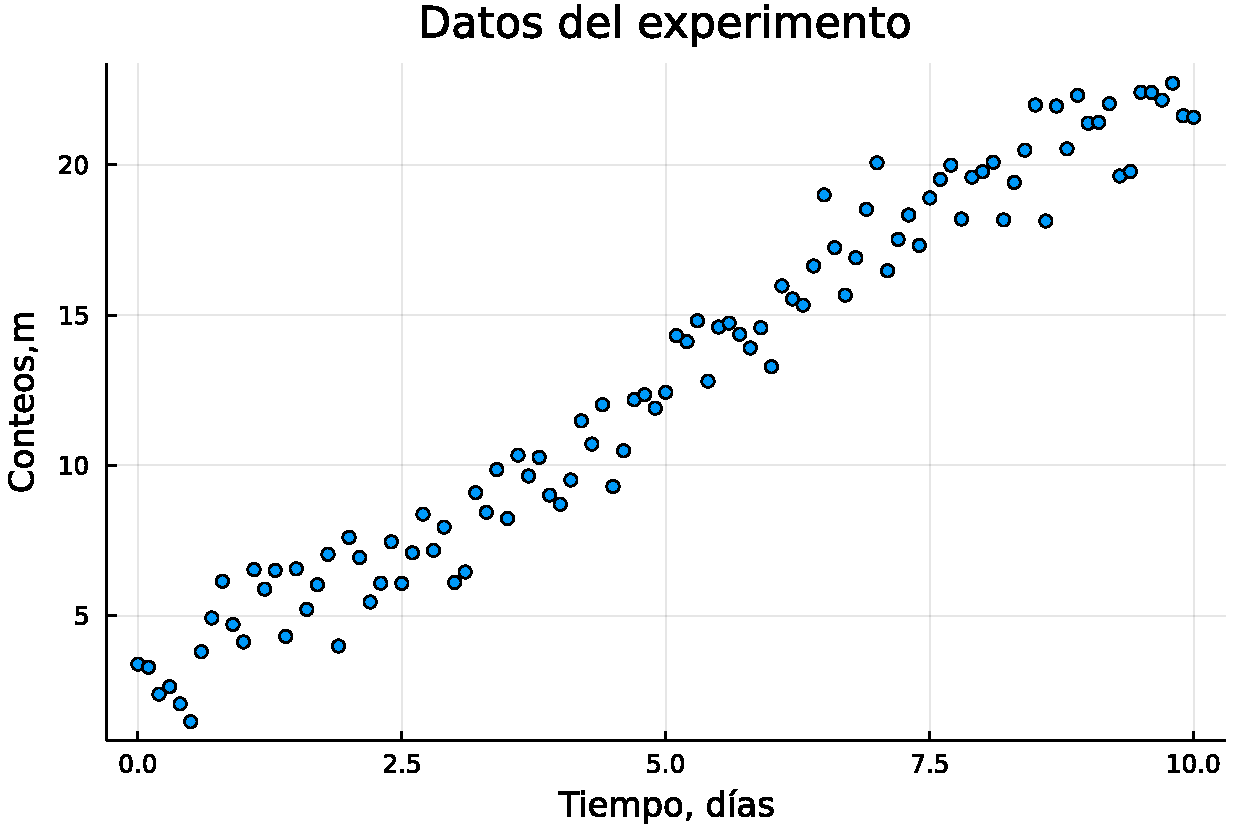
\includegraphics[scale=0.4]{images/bacterias_experimento.pdf}

	\end{figure}
\end{frame}

\begin{frame}
	\begin{itemize}
		\item Queremos modelar el crecimiento de una población de bacterias.
		\item Se asume el siguiente modelo de crecimiento poblacional,
		
		\[\dfrac{dN}{dt} = \alpha N (1-\beta N)\]
		
		donde $\alpha > 0$ es la tasa de crecimiento debida a la división celular y $\beta >0$ mide la reducción en la trasa de crecimiento debido a la aglomeración.
		
		\begin{center}
			\textbf{¿Cómo inferimos los parámetros de este modelo?}
		\end{center}
	\end{itemize}
\end{frame}

\begin{frame}
	Asumamos un error de medición alrededor del valor verdadero:
	\[N^*(t) \sim \text{normal}(N(t),\sigma)\]	
	
	donde:
		\begin{itemize}
			\item $N^*(t)$ es el conteo de bacterias en el tiempo $t$.
			\item $N(t)$ es la solución de la ODE en el tiempo $t$ (número verdadero de bacterias en la placa).
			\item $\sigma >0$ mide la magnitud del error de medición alrededor del valor verdadero.
		\end{itemize}
\end{frame}

\begin{frame}
	\begin{figure}
		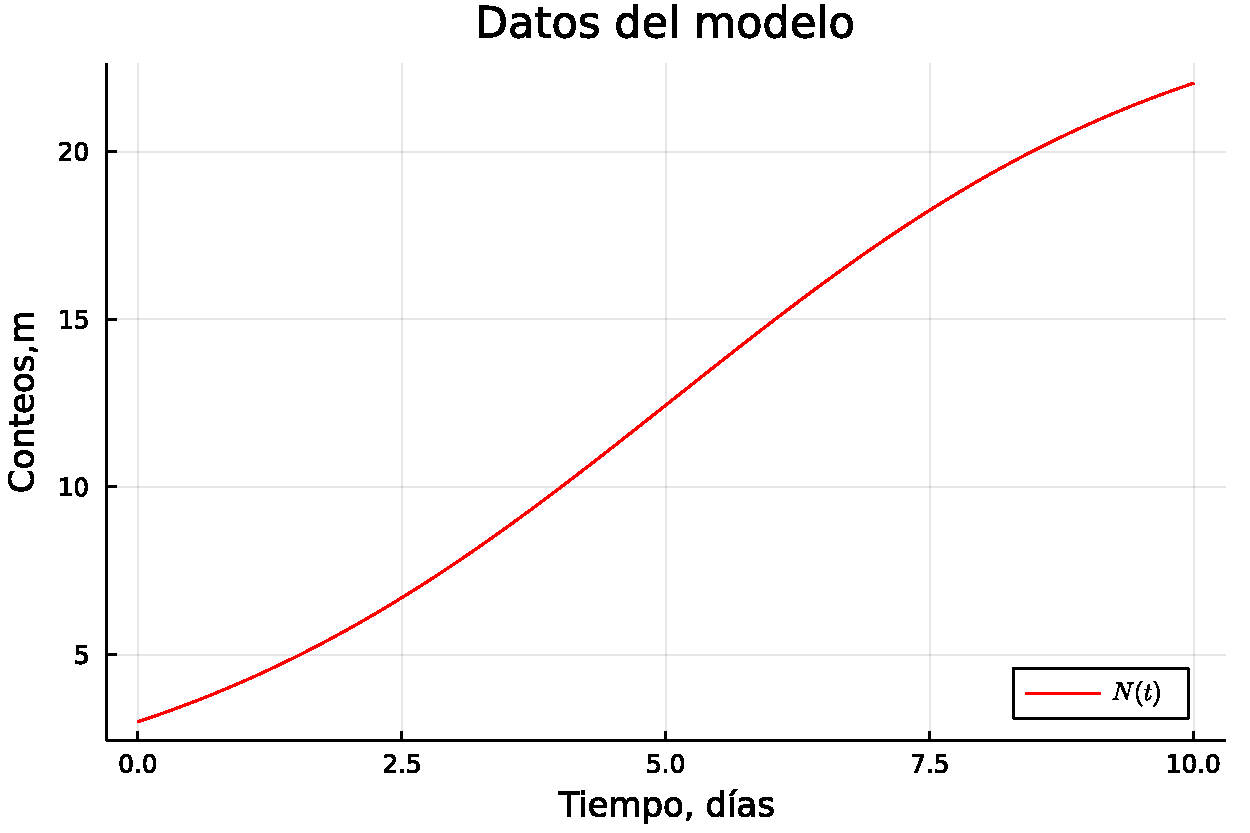
\includegraphics[scale=0.5]{images/bacterias_modelo.pdf}
		\caption{Número verdadero de bacterias, $N(t)$}
	\end{figure}
\end{frame}

\begin{frame}

Superposición de distribución de muestreo que representa el error de medición y de los datos experimentales.

	\begin{figure}
		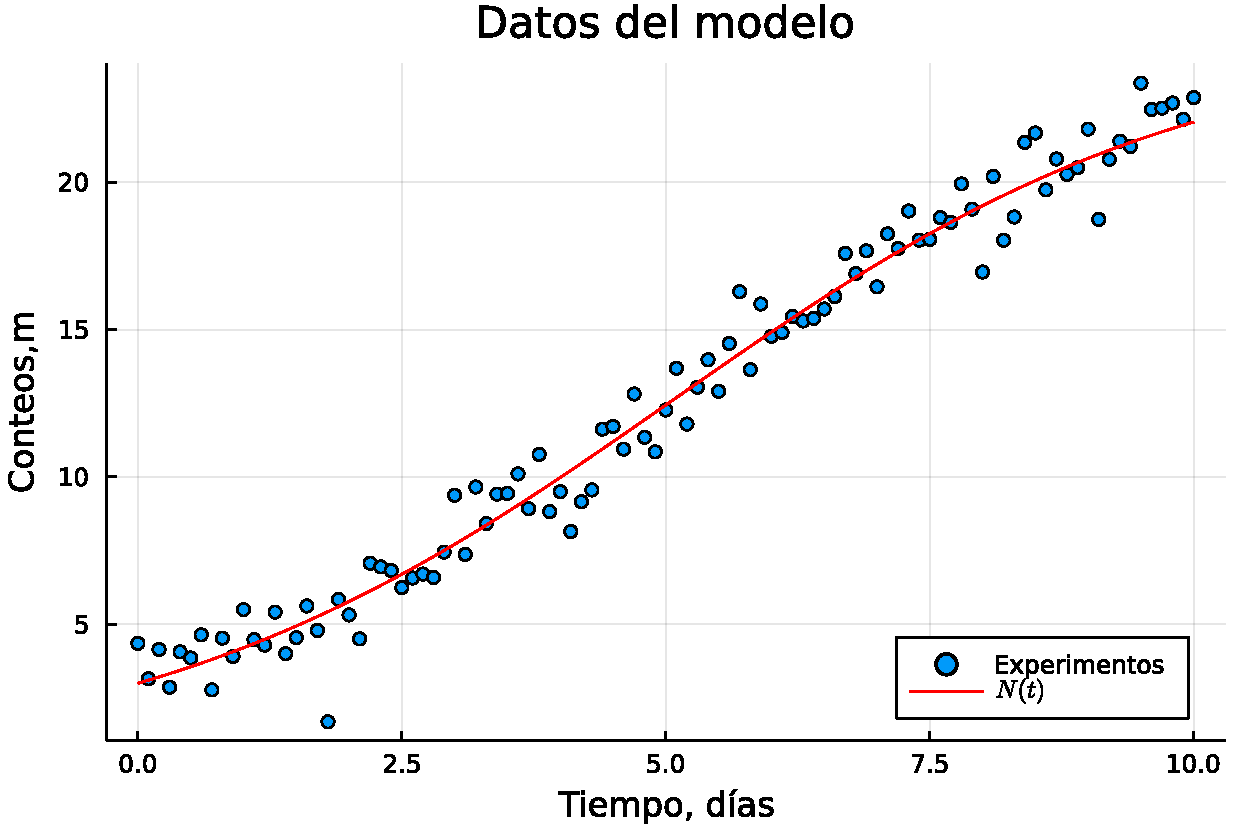
\includegraphics[scale=0.5]{images/bacterias_modelo_experimentos.pdf}
	\end{figure}
\end{frame}

\begin{frame}
Dado que estamos usando la distribución normal,

\[N^*(t) \sim \text{normal}(N(t),\sigma)\]

la verosimilitud de las observaciones es

\[L(N(t),\sigma) = \prod_{t=t_1}^T  \dfrac{1}{\sqrt{2\pi\sigma^2}} \exp{\Big[  \dfrac{-(N^*(t)-N(t))^2}{2\sigma^2}\Big]}\]

\begin{center}
	\textbf{¿Cómo calculamos $N(t)$?}
\end{center}

		\[\dfrac{dN}{dt} = \alpha N (1-\beta N)\]

\end{frame}

\begin{frame}

Cualquier solución de $N(t)$ -exacta o numérica- depende de los parámetros del modelo de ODE. En este caso,

\[N(t) = f(t,\alpha,\beta)\]

\begin{center}
	\textbf{¿Cómo integramos los datos observados para estimar estos parámetros?}
\end{center}

\end{frame}

\begin{frame}{Inferencia bayesiana}
	\begin{itemize}
		\item En un contexto de inferencia bayesiana, donde se tiene un modelo muestral $Y \sim p(y|\theta)$ y una distribución inicial $p(\theta)$, la distribución final se calcula de la siguiente forma:
		
		 \begin{equation*}
		 	p(\theta | y) =  \dfrac{p(y | \theta)p(\theta)}{\int p(\theta{'}) p(y|\theta{'})d\theta{'}}
		 \end{equation*} 
		\item Aún descartando el denominador (el cual se puede interpretar como un factor de escalamiento que hace que la función integre a 1), el cálculo analítico de $p(\theta | y) $, en la mayoria de las ocasiones, es complicado.
	\end{itemize}
	
\end{frame}


\begin{frame}\small
	\begin{itemize}
		\item Hay distintas técnicas para calcular $p(\theta | y) $ (aproximación de Laplace, métodos de cuadratura, etc), pero por la capacidad de cómputo disponible las técnicas de simulación de Monte Carlo vía cadenas de Markov (MCMC) han sido mayormente utilizadas.
		\item La idea de MCMC es \textbf{construir una cadena de Markov que sea fácil de simular (a través de un proceso de muestreo) y cuya distribución de equilibrio corresponda a la distribución final de interés}.
	\end{itemize}
\end{frame}

\begin{frame}
	\begin{itemize}
		\item En el contexto de nuestro problema,
		\begin{itemize}
			\item $p(\theta)$ puede como la distribución inicial de los parámetros del modelo de ODE, 
			\item $p(y|\theta)$ (el modelo muestral o distribución de verosimilitud) representa el modelo de ODE. 
		\end{itemize}	
		
		\item Podemos utilizar las técnicas de MCMC para construir la distribución $p(\theta|y)$, de los parámetros del modelo de ODE.  
	\end{itemize}
\end{frame}

\begin{frame}{Turing}
\textbf{Turing} es un lenguaje de programación probabilística de propósito general para una inferencia bayesiana robusta y eficiente. Las características actuales incluyen:

	\begin{itemize}
		\item Programación probabilística de propósito general con una interfaz de modelado intuitiva;
		\item Muestreo de Monte Carlo hamiltoniano (HMC) robusto y eficiente para distribuciones posteriores diferenciables;
		\item 
Muestreo de partículas MCMC para distribuciones posteriores complejas que involucran variables discretas y flujo de control estocástico; e
		\item 
Inferencia composicional a través del muestreo de Gibbs que combina partículas MCMC, HMC y paseo aleatorio MH (RWMH).
	\end{itemize}
\end{frame}


%%%%%%%%%%%%%%%%%%%%%%%%%%%%%%%%%%%%%%%%%%%%%%%%%%%%%%%%%%%%%%%%%%%%%%%%%%%%%%%%%%%%%%%%%%%%
\begin{frame}{Algoritmo de Metrópolis }

\begin{itemize}
	\item Considerando el caso en que se tiene un modelo muestral $Y \sim p(y|\theta)$ y una distribución inicial $p(\theta)$.
	\item La distribución final es difil de calcular por la integral en el denominador:
		 \begin{equation}
		 	p(\theta | y) =  \dfrac{p(\theta)p(y | \theta)}{\int p(\theta{'}) p(y|\theta{'})d\theta{'}}
		 \end{equation}
	\item Si se pudiera obtener muestras de $p(\theta|y)$, se podría generar $\theta^{(1)},\theta^{(2)}, \hdots, \theta^{(S)} \sim \text{i.i.d}. p(\theta | y)$ y obtener aproximaciones con el método de Monte Carlo.
	\item El problema es cuando no se pueden obtener muestras directamente de $p(\theta | y)$.
\end{itemize}
\end{frame}


\begin{frame}
	\begin{itemize}
		\item En términos de aproximar la distribución posterior, lo crítico no es tener muestras i.i.d. de $p(\theta |y)$ sino que poder construir una gran colección de valores de $\theta$, cuya distribución empírica aproxime $p(\theta | y)$
		\item Suponiendo que se cuenta con una colección $\lbrace \theta^{(1)},\theta^{(2)}, \hdots, \theta^{(s)}\rbrace$ a la cual queremos agregar un valor nuevo $\theta^{s+1}$.
		\item Se considera agregar un valor $\theta^{*}$ que es cercano a $\theta^{s}$.
		\item \textbf{¿Qué regla de decisión utilizamos?}
	\end{itemize}
\end{frame}

\begin{frame}
	\begin{itemize}
				\item Si $p(\theta^{*}|y) > p(\theta^{(s)}|y)$, se prefieren más valores de $\theta^{*}$ en el conjunto que los valores de $\theta^{(s)}$.
				\item Dado que $\theta^{(s)}$ ya está en el conjunto, entonces parece que deberíamos incluir también a $\theta^{*}$.
		\item En el caso contrario, si $p(\theta^{*}|y) < p(\theta^{(s)}|y)$ no es necesario incluir $\theta^{*}$.
		\item Así, parece que la decisión de incluir o no a $\theta^{*}$ depende de la comparación entre $p(\theta^{*}|y)$ y $p(\theta^{(s)}|y)$. 
		\item Afortunadamente, esta comparación se puede hacer incluso si no podemos calcular $p(\theta | y)$
	\end{itemize}
	\begin{equation}
	r = \dfrac{p(\theta^{*} | y)}{p(\theta^{(s)} | y)} = \dfrac{p(y | \theta^{*}) p(\theta^{*})}{p(y)} \dfrac{p(y)}{p(y | \theta^{(s)})p(\theta^{(s)})} = \dfrac{p(y | \theta^{*}) p(\theta^{*})}{p(y | \theta^{(s)})p(\theta^{(s)})}
	\end{equation}
\end{frame}

\begin{frame}
Habiendo calculado $r$, ¿qué tenemos que hacer?

	\begin{itemize}
		\item Si $r >1$:
			\begin{itemize}
				\item \textbf{Intuición}: Dado que $\theta^{(s)}$ ya está en el conjunto, debemos incluir a $\theta^{*}$ ya que tiene una probabilidad mayor que $\theta^{(s)}$.
				\item \textbf{Decisión}: Aceptar $\theta^{*}$ en nuestro conjunto, \textit{i.e.} definir $\theta^{s+1}=\theta^{*}$.
			\end{itemize}
		\item Si $r < 1$:
			\begin{itemize}
				\item \textbf{Intuición}: La frecuencia relativa de valores $\theta$ en el conjunto que es igual a $\theta^{*}$, comparado con aquellos valores iguales a $\theta^{(s)}$ está dada por la expresión $\dfrac{p(\theta^{*} | y)}{p(\theta^{(s)}|y)} = r$. Esto significa que por cada instancia de $\theta^{(s)}$, deberíamos tener sólo una fracción de valores $\theta^{*}$.
				\item \textbf{Decisión}:  Definir $\theta^{s+1}$ igual a $\theta^{*}$ o $\theta^{(s)}$ con probabilidad $r$ y $1-r$ respectivamente.  
			\end{itemize}
	\end{itemize}
\end{frame}

\begin{frame}{Algoritmo Metropolis} 
	\begin{itemize}
		\item Lo anterior es la intuición básica del algoritmo de \textbf{Metropolis}.
		\item El algoritmo de Metropolis procede al muestrear un valor $\theta^{*}$ cercano al valor actual $\theta^{(s)}$ usando una distribución simétrica  $J(\theta^{*} | \theta^{(s)})$.
		\item En este contexto, simetría significa que $J(\theta_b | \theta_a) = J(\theta_a | \theta_b)$, \textit{i.e.} la probabilidad de proponer  $\theta^{*} = \theta_b$ dado que $\theta^{(s)}=\theta_a$ es igual a la probabilidad de proponer $\theta^{*} = \theta_a$ dado que $\theta^{(s)}=\theta_b$.
		\item Algunos ejemplos de $J(\theta^{*} | \theta^{(s)})$ son :
			\begin{itemize}
				\item $J(\theta^{*} | \theta^{(s)}) = \text{uniform}(\theta^{(s)}- \delta,\theta^{(s)} + \delta )$
				\item $J(\theta^{*} | \theta^{(s)}) = \text{normal}(\theta^{(s)},\delta^{2})$
			\end{itemize}
		\item El valor del parámetro $\delta$ generalmente se elige para hacer que el algoritmo se ejecute de manera eficiente.
	\end{itemize} 
\end{frame}

\begin{frame}
	\begin{itemize}
		\item \textbf{Habiendo obtenido un valor propuesto} $\theta^{*}$ \textbf{se añade al conjunto este valor o a una copia de } $\theta^{(s)}$ \textbf{, dependiendo de la proporción } $ r = \dfrac{p(\theta^{*} | y)}{p(\theta^{(s)}|y)}$
	\end{itemize}
\end{frame}


\begin{frame}
De forma específica, dado $\theta^{(s)}$, el algoritmo Metropolis genera un valor $\theta^{(s+1)}$ de la siguiente forma:

	\begin{enumerate}
		\item Tomar una muestra $\theta^{*} \sim J(\theta | \theta^{(s)})$
		\item Calcular la proporción de aceptación
			\begin{equation*}
					r = \dfrac{p(\theta^{*} | y)}{p(\theta^{(s)} | y)} = \dfrac{p(y | \theta^{*}) p(\theta^{*})}{p(y | \theta^{(s)})p(\theta^{(s)})}
			\end{equation*}
		\item Sea
		\begin{equation}
		  \theta^{(s+1)} =
    		\begin{cases}
      			\theta^{*} \qquad \text{con probabilidad $\min(r,1)$}\\
  	  			\theta^{(s)} \qquad \text{con probabilidad $1- \min(r,1)$}
    		\end{cases}       
		\end{equation}

	\end{enumerate}
	
	El paso 3 se puede obtener al tomar una muestra $u \sim \text{uniform}(0,1)$ y definir $\theta^{s+1}= \theta^{*}$ si $u < r$ y $\theta^{s+1}= \theta^{\theta^{(s)}}$ en otro caso. 
\end{frame}

%%%%%%%%%%%%%%%%%%%%%%%%%%%%%%%%%%%%%%%%%%%%%%%%%%%%%%%%%%%%%%%%%%%%%%%%%%%%%%%%%%%%%%%%%%%%


\begin{frame}
	\begin{center}
		{\huge \textbf{¡Vamos a programar!}}
	\end{center}
\end{frame}


\begin{frame}
	\begin{figure}
		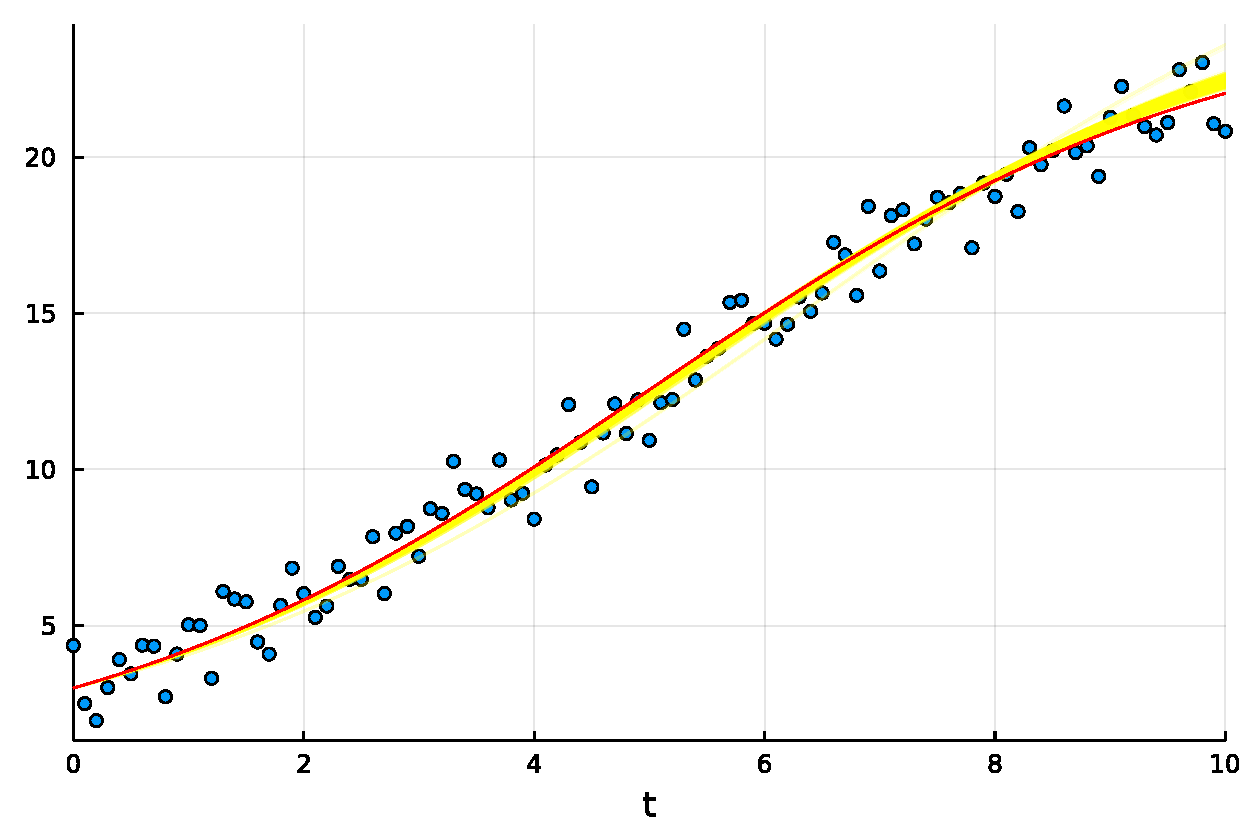
\includegraphics[scale=0.5]{images/final_plot.pdf}
	\end{figure}
	La distribución posterior (línea amarilla) reproduce con bastante precisión la solución \textit{verdadera} del ODE.
\end{frame}

\begin{frame}
	\begin{figure}
		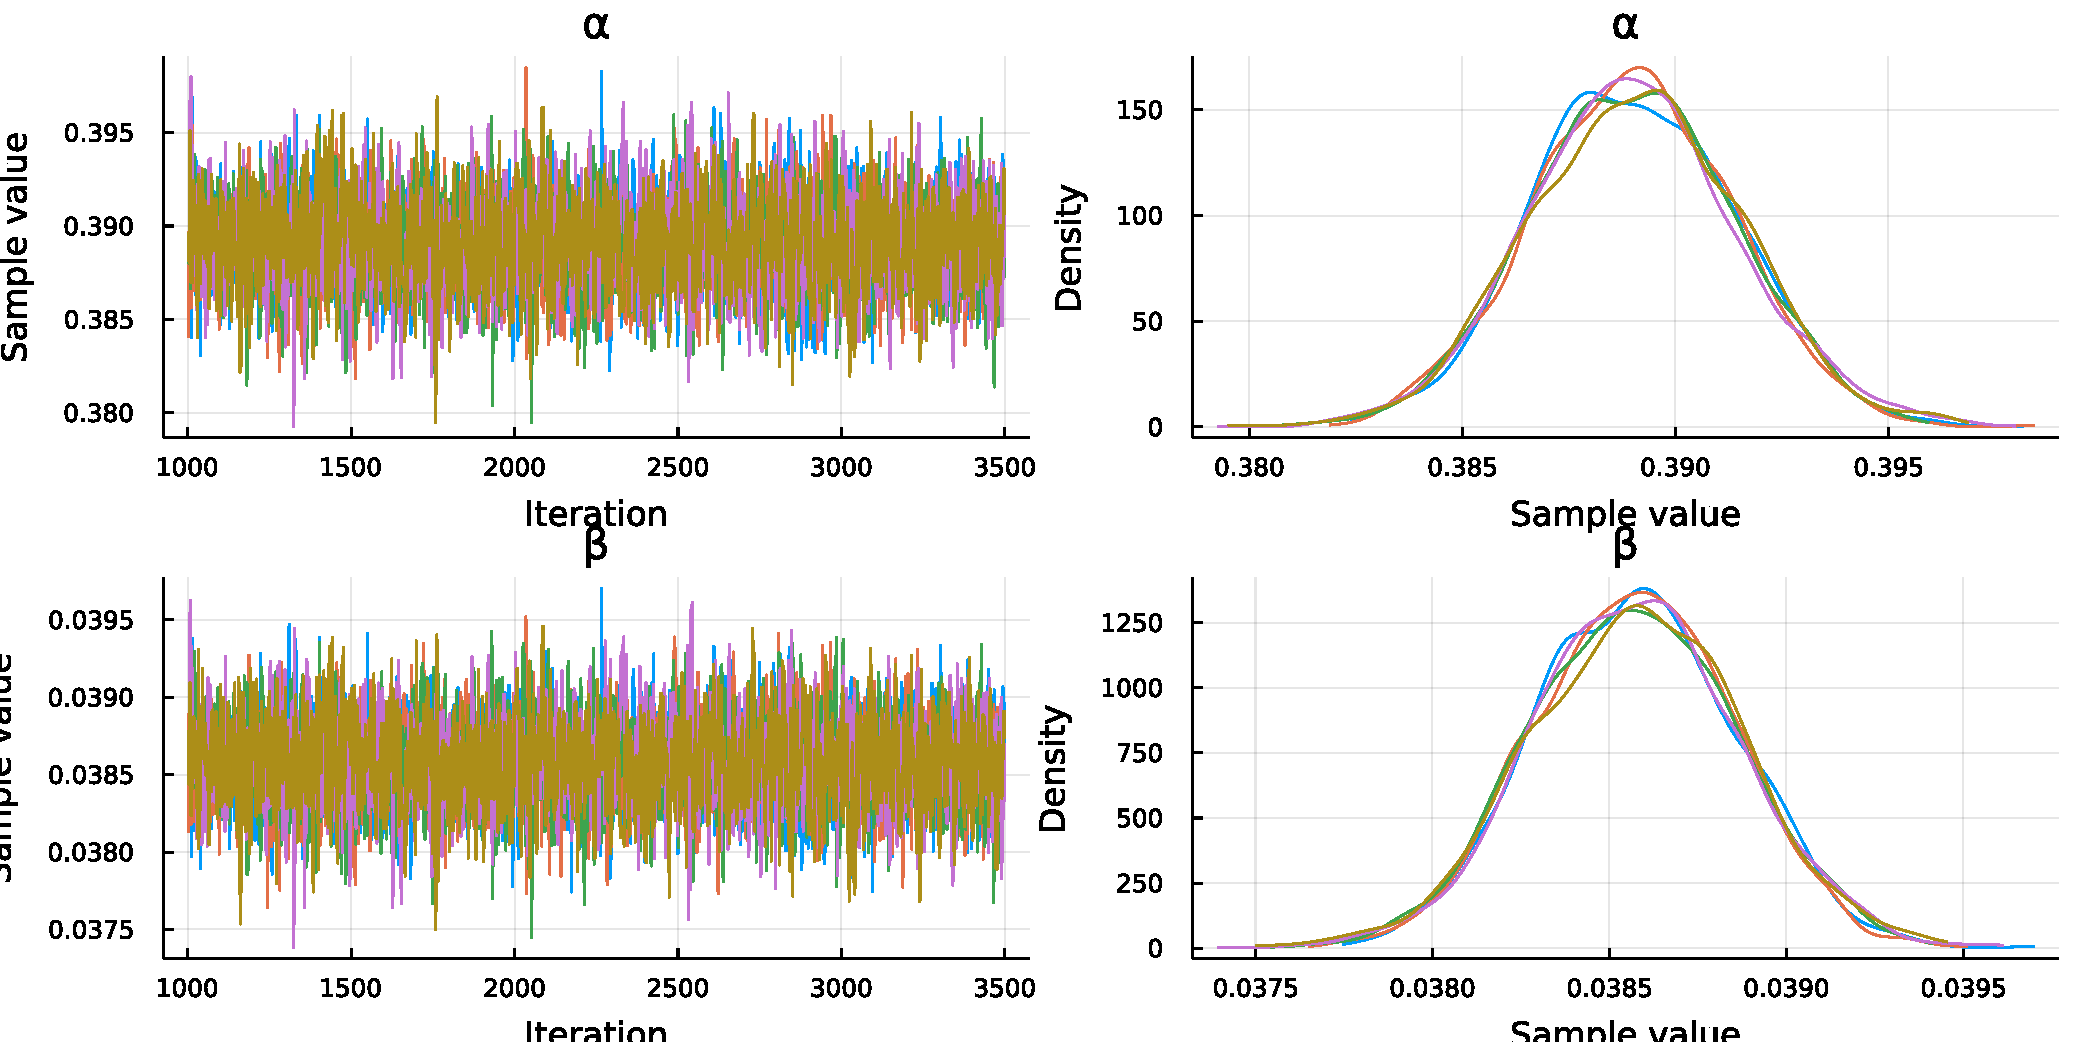
\includegraphics[scale=0.35]{images/chain_resultados.pdf}
	\end{figure}
\end{frame}
\end{document}